\documentclass[11pt]{article}
\usepackage[utf8]{inputenc}
\usepackage[T1]{fontenc}
\usepackage{lmodern}
\usepackage[margin=1in]{geometry}
\usepackage{microtype}
\setlength{\emergencystretch}{3em}  % avoid margin spills from unbreakable \texttt model names
\usepackage{amsmath,amssymb}
\usepackage{booktabs}
\usepackage{graphicx}
\usepackage{multirow}
\usepackage{array}
\usepackage{xcolor}
\usepackage{enumitem}
\usepackage{caption}
\usepackage[numbers,sort&compress]{natbib}
\usepackage[hidelinks]{hyperref}

\graphicspath{{../figures/}}

% placeholder for citations to be filled after the literature pass; keeps the draft compiling
\newcommand{\todocite}[1]{\textcolor{blue}{[\,#1\,]}}
\newcommand{\todo}[1]{\textcolor{red}{[TODO: #1]}}
\newcommand{\result}[1]{#1}  % design numbers, now locked from the data
\newcommand{\rqthree}{A comprehension study across a ladder of student models confirms the
practical upshot: a plain explanation lifts the weakest model's accuracy by roughly sixteen
points, but adding an analogy on top yields no measurable gain over the explanation for any of
them.}

\title{\bfseries Generating and Evaluating STEM Teaching Analogies with Small Language Models}

\author{\textbf{Sriharsha Meduri}\textsuperscript{a} \quad Mohit Pratap Singh Rathore\textsuperscript{a} \quad
  Gunveer Kalsi\textsuperscript{a} \quad Pratap Chandra Mandal\textsuperscript{b} \\[3pt]
  \small \textsuperscript{a}Oviqo \qquad \textsuperscript{b}Indian Institute of Management Shillong \\[2pt]
  \small Correspondence: \texttt{sriharshameduri07@gmail.com}}
\date{\today}

\begin{document}
\pagenumbering{arabic}
\pagestyle{plain}
\maketitle
\thispagestyle{plain}

\begin{abstract}
\noindent
Analogies help teachers make abstract STEM concepts concrete, and language models
can now generate them on demand. This raises two practical questions: \emph{how}
should one prompt for good analogies, and \emph{how} can analogy quality be evaluated
at scale without a human rating every item? We study both using only small, open
models on a single consumer GPU, with no paid API and no human annotation. For
\result{64} school-level concepts across four subjects, three open models generate
analogies under four source-domain strategies (unconstrained, everyday, sports,
cooking), and a four-model panel evaluates each with a purpose-built five-dimension
rubric (SAQR). Because small models score leniently and inconsistently, we take
\emph{comparative ranking} as the primary signal and validate the panel against
planted analogies of known quality. Constraining the source domain confers no
advantage over unconstrained generation: equivalence tests place all four strategies
within a small margin. Judged quality is highly predictable ($R^2 = 0.72$), but from
length and subject, not strategy, a verbosity bias we quantify. The panel screens out
planted-wrong analogies almost perfectly yet barely agrees when ranking good ones; a plain
explanation lifts weak students' accuracy while an added analogy does not; and a preliminary Hindi
replication is consistent, though the automated evaluation does not carry over. A judge twice the
panel's size sheds the verbosity bias and resolves a small but significant advantage for
unconstrained generation, so the equivalence partly reflects the small panel's own limitation. The paper contributes a reusable, fully automated, reproducible
protocol and a candid account of automated evaluation's failure modes and their mitigations.
\end{abstract}

\section{Introduction}
\label{sec:intro}
A good analogy can turn an abstract STEM concept into something a student already
understands. Comparing electric current to water in a pipe, or a chemical
equilibrium to a crowded two-way bridge, lets a learner import familiar structure
onto unfamiliar ideas, and decades of work in the learning sciences treat this
mapping of relations as central to how people understand new material
\citep{gentner1983structure,duit1991role}. Analogies are not a panacea: reviews of
classroom use find that their benefit is real but conditional, and that a
carelessly chosen analogy can just as easily plant a misconception a student then
has to unlearn \citep{dagher1995review,clement1993bridging}. The quality of the
analogy, and its fit to the concept, is what matters.

Large language models change the economics of producing such analogies. A teacher
can now ask a model for ten analogies for photosynthesis in seconds, and early
studies show that model-generated analogies can help learners, particularly when
a teacher curates them \citep{bhavya2022analogy,shao2025unlocking}. This
possibility raises two practical questions that the present paper addresses
together. First, \emph{how should one prompt} a model to obtain good analogies:
does it help to constrain the analogy's source domain (``explain it with a sports
analogy''), or is the model's own unconstrained choice at least as good? Second,
and prerequisite to answering the first at any scale, \emph{how can analogy
quality be measured} without a human expert rating every candidate? The natural
answer, to have a language model judge the analogies, inherits the known
reliability problems of LLM-as-a-judge evaluation, including leniency, verbosity
preference, self-preference, and sensitivity to the order in which options are
presented \citep{zheng2023judging}.

We study both questions using only small, openly available models that run on a
single consumer GPU, with no paid API and no human annotation in the loop. This
choice is deliberate: it keeps the whole protocol reproducible on commodity
hardware and forces us to confront, rather than paper over, the reliability limits
of automated evaluation. Along the way we find that those limits bite in two
concrete places: a capable ``student'' model ceilings on our comprehension
questions because it already knows the material, and small judge models rate
almost everything highly and are easily biased by option order. We develop
mitigations (a weak-to-strong student ladder, comparative ranking with shuffled
labels, and a validation probe of planted known-quality analogies) that keep the
measurements honest. This fully-automated regime is a deliberate scope, not a claim
that automated proxies replace human teachers and learners: it is the setting a
resource-constrained educator or a large-scale content pipeline actually faces, and the
one in which a cheap, reproducible screening protocol is most useful. Human validation is
a complementary next step, which we discuss in Section~\ref{sec:limitations}, not a
prerequisite for the questions we ask here.

\paragraph{Research questions.}
\begin{description}[leftmargin=2.2em,style=nextline]
  \item[RQ1.] Do analogy \emph{generation strategies} (the source domain the
    model is asked to draw the analogy from) differ in the quality of the
    analogies they produce, as judged by an automated multi-model panel?
  \item[RQ2.] What do the automated \emph{judges reward}? Can an analogy's judged
    score be predicted from cheap features, and what does that reveal about the
    judges' biases rather than about true quality?
  \item[RQ3.] Does an added analogy carry information that measurably improves a
    proxy ``student'' model's answers to conceptual questions, and how does that
    depend on the student's capability?
  \item[RQ4.] Do these findings \emph{replicate in Hindi}, a mid-resource
    language, and how far do small open models degrade when generating and
    judging analogies outside English?
\end{description}

\paragraph{Research objectives.} Each question is paired with a research objective (RO) that
operationalises it, so that every objective is answered by a specific analysis reported later in
the paper.
\begin{description}[leftmargin=2.2em,style=nextline]
  \item[RO1.] To measure and compare, with an automated multi-model panel, the instructional
    quality of analogies generated under different source-domain prompting strategies
    (addresses RQ1; Section~\ref{sec:results:rq1}).
  \item[RO2.] To audit the automated judges by predicting their scores from cheap features and
    quantifying the biases, such as verbosity, that threaten automated quality measurement
    (addresses RQ2; Section~\ref{sec:results:rq2}).
  \item[RO3.] To test whether an added analogy improves a proxy student model's answers to
    conceptual questions, and how this depends on the student's capability
    (addresses RQ3; Section~\ref{sec:results:rq3}).
  \item[RO4.] To assess how far both the generation findings and the automated-evaluation protocol
    transfer from English to Hindi, a mid-resource language
    (addresses RQ4; Section~\ref{sec:results:rq4}).
\end{description}

\paragraph{Contributions.} We organise the contributions along three pillars: academic and
research, industry and managerial, and society.

\emph{Academic and research.} (i)~The STEM Analogy Quality Rubric (SAQR), a five-dimension rubric
for instructional analogies grounded in the learning-sciences literature, together with a
\emph{judge-validation probe} of planted known-quality analogies that objectively tests whether an
automated judge can tell good analogies from bad ones. (ii)~Empirical findings on prompting strategy
(no reliable source-domain effect), on what the automated judges actually reward (surface length and
subject, a bias we quantify in this instructional setting), on how an added analogy interacts with a
proxy student's capability, and on how far these carry into Hindi rather than only English.
(iii)~A candid account of two failure modes of automated evaluation (student ceiling effects, and
lenient, position-biased judges) and the mitigations (weak-student gradients, comparative ranking,
label shuffling, probe validation) that keep the protocol honest.

\emph{Industry and managerial.} A fully automated, reproducible protocol for generating and
screening STEM analogies with small open models on a single consumer GPU, with no paid API or human
annotation, that an educational-technology team or a content pipeline can adopt directly. It yields
actionable guidance: let a capable model choose the analogy's domain rather than engineering
source-domain constraints, treat a small-model panel as a cheap \emph{screen} rather than a
fine-grained ranker and validate it against known-quality anchors, and scale the judge only when
finer discrimination is needed.

\emph{Society.} By requiring neither paid services nor specialised hardware, the protocol lowers the
barrier for resource-constrained teachers, schools, and education regulators to vet automatically
generated teaching material before it reaches learners. The Hindi study also surfaces an equity
concern with practical weight: at this model scale automated evaluation is an English-first tool, so
learners and educators working in mid-resource languages are currently underserved, which we name as
a target for the field.

\paragraph{How this study differs from prior work.} SAQR is a new rubric we introduce for this
problem, not a pre-existing standard, and the study as a whole occupies a combination that earlier
work does not. Prior evaluations of language-model-generated analogies either rely on human raters or
paid frontier judges \citep{shao2025unlocking,zheng2023judging}, target analogy \emph{identification
or solving} rather than the quality of instructional \emph{generation}
\citep{jiayang2023storyanalogy,ye2024analobench}, or report judge scores without testing whether the
judge can actually distinguish good analogies from bad. We instead evaluate instructional generation
with a purpose-built rubric using only small open models, and we validate the judges against planted
known-quality analogies, quantify their biases, tie quality to a comprehension outcome across a
student-capability gradient, and test transfer to Hindi, while being explicit about where the
automation fails. It is this combination, not any single component, that is new.

\section{Related Work}
\label{sec:related}

\paragraph{Analogy in the learning sciences.}
Gentner's structure-mapping theory frames an analogy as a mapping of \emph{relations}
(not surface features) from a familiar base to an unfamiliar target, and it explains
why some analogies illuminate while others merely decorate \citep{gentner1983structure}.
In science education specifically, analogies and metaphors are ubiquitous, and their
instructional value has been studied for decades \citep{duit1991role}. The picture is
mixed: reviews find that analogies help under the right conditions but can also seed
durable misconceptions when the mapping breaks down in a place the learner over-extends,
which motivated structured classroom techniques such as bridging analogies and explicit
mapping of correspondences \citep{dagher1995review,clement1993bridging}. This literature
grounds two of our rubric dimensions, conceptual accuracy and the \emph{absence of
misleading simplification}, as the qualities that most distinguish a helpful analogy
from a harmful one.

\paragraph{Computational and LLM-based analogy generation.}
Analogy has long been a target for natural language processing, historically through
word-level proportional analogies and, more recently, through free-form generation with
LLMs. \citet{bhavya2022analogy} showed that prompting can elicit serviceable analogies
from instruction-tuned models, and subsequent work has built corpora and benchmarks for
story-level and abstract analogical reasoning \citep{jiayang2023storyanalogy,ye2024analobench}.
These efforts largely evaluate whether models can \emph{identify} or \emph{solve} analogies;
we instead study how the \emph{prompting strategy} shapes the quality of generated
instructional analogies, and how that quality can be measured automatically.

\paragraph{LLMs as instructional-content generators.}
Language models are increasingly used to draft explanations, questions, feedback, and
other teaching materials \citep{kasneci2023chatgpt}. Closest to our setting,
\citet{shao2025unlocking} evaluated LLM-generated analogies with high-school students and
teachers, reporting comprehension gains, especially in biology, but also a need for
teacher curation to prevent over-reliance. Their study centres human judgement; ours is
complementary, asking how far a \emph{fully automated} pipeline of small open models can
generate and screen analogies before a human is involved, and being explicit about where
that automation is and is not trustworthy.

\paragraph{LLM-as-a-judge and its reliability.}
Using a strong model to score generated text correlates well with human preference in
aggregate but is subject to well-documented biases: position/order bias, verbosity bias,
and self-enhancement bias, among others \citep{zheng2023judging}. Most of this evidence
concerns large frontier judges; we find the problems are sharper with the small local
models we are constrained to, which additionally exhibit strong leniency (rating nearly
everything highly) and, in ranking, a tendency to default to presentation order. Our
response adapts standard LLM-as-a-judge practice to a small-model, education-specific
setting: comparative ranking with per-item label shuffling, exclusion of self-judgements,
and an objective judge-validation probe of planted good/wrong analogies. It quantifies when
the resulting scores can and cannot be trusted.

\section{The STEM Analogy Quality Rubric (SAQR)}
\label{sec:rubric}
We designed a compact rubric for judging an analogy \emph{as a teaching aid for a
specific concept}, rather than as free-standing text. SAQR has five dimensions,
each scored from 1 (poor) to 5 (excellent) against anchored descriptions:
\emph{conceptual accuracy} (do the important relationships in the concept
correspond to matching relationships in the analogy?), \emph{clarity} (is it
easy to follow and does it actually aid understanding?), \emph{memorability} (is
it vivid and concrete enough to be remembered?), \emph{absence of misleading
simplification} (does it avoid planting a misconception?), and \emph{overall
usefulness}. The full rubric with all anchors is given in
Appendix~\ref{app:rubric}. The dimensions were chosen to separate the two ways an
analogy can fail that matter most in teaching (being \emph{wrong}, that is, low
conceptual accuracy, or \emph{subtly misleading}, that is, low non-misleading
score) from the ways it can merely be ineffective (low clarity or
memorability). Empirically the five dimensions are moderately correlated but not
redundant (mean pairwise $r = 0.31$ across all judgments), and the
absence-of-misleading-simplification dimension is close to orthogonal to the rest
($r$ between $-0.07$ and $0.11$ with conceptual accuracy, memorability, and overall
usefulness). Whether an analogy misleads is therefore \emph{not} captured by whether
it is clear, accurate, or memorable, which is exactly why it earns a place as its own
dimension.

\section{Method}
\label{sec:method}

\subsection{Overview}
The study has one manipulated variable (the analogy \emph{generation
strategy}) and a fixed pipeline of automated measurements around it. For each
concept we hold the standard textbook explanation constant and vary only the
prompt used to elicit an analogy. Every generated analogy is then (a) ranked
against its siblings by a judge panel, (b) scored on the SAQR rubric by the same
panel, and, for a subset of concepts with multiple-choice questions, (c) placed
in front of ``student'' models of differing capability to measure a
comprehension outcome. All generation and evaluation is performed by small open
models served locally through Ollama on a single NVIDIA GTX~1650 (4\,GB);
no external API or human annotation is used at any stage.

\subsection{Concept dataset}
\label{sec:method:concepts}
We authored \result{64} school-curriculum concepts, balanced across four subjects
(Physics, Chemistry, Mathematics, Biology; \result{16} each) and spanning grades
8--12. Each concept carries a concise, curriculum-accurate standard explanation
(mean \result{62} words). A \result{16}-concept subset additionally carries four
four-option multiple-choice questions ($\result{64}$ questions in total),
written to probe conceptual understanding and transfer rather than verbatim
recall; these support the comprehension study (RQ3). Concept content (the
explanations and the questions with their verified keys) was authored and checked
by the researcher; only the analogies are model-generated, so that the
manipulated variable is cleanly separated from the fixed teaching content. The
full concept list appears in Appendix~\ref{app:concepts}.

\subsection{Analogy generation strategies (the independent variable)}
\label{sec:method:generation}
Each analogy is produced by prompting a generator model with a system role of an
expert STEM teacher and a user prompt that supplies the concept, its standard
explanation, and one \emph{strategy instruction} constraining the source domain
of the analogy. The four strategies are: \textbf{free} (any source domain, the
unconstrained reference), \textbf{everyday} (ordinary daily-life objects and
routines), \textbf{sports} (sports, games, or physical play), and
\textbf{cooking} (cooking, baking, or the kitchen). The prompt asks for a single
analogy of two to four sentences that ``maps correctly onto the concept.'' To
check that the choice of generator does not drive the result, we run the full strategy set with
three open models as generators (\texttt{qwen2.5:3b}, \texttt{llama3.2:3b}, and
\texttt{gemma2:2b}), yielding $\result{64}\times4\times3=\result{768}$ analogies.
Generation uses temperature 0.7 with a fixed per-item seed; every prompt and
completion is logged verbatim for reproducibility.

\subsection{Automated evaluation}
\label{sec:method:eval}
Small local models turn out to be unreliable \emph{absolute} scorers: they cluster
at the top of the scale and anchor it differently from one another
(Section~\ref{sec:results:agreement}). We therefore use two complementary
evaluation channels and treat the comparative one as primary.

\paragraph{Comparative ranking (primary).}
For each concept and each generator, a judge is shown all four strategy analogies
at once, with their presentation letters \emph{shuffled per (judge, concept)} to
control position bias, and is asked to rank them from best (1) to worst (4) as
teaching aids, each rank used once. Rankings are parsed as permutations; invalid
outputs (missing or duplicated ranks) are discarded. A model never ranks
analogies it generated itself (self-preference control). The panel comprises
\texttt{qwen2.5:3b}, \texttt{llama3.2:3b}, \texttt{gemma2:2b}, and
\texttt{phi3.5}, so each analogy set is ranked by the three panel members that
did not generate it. We report the mean rank per strategy, a Friedman test across
strategies (using per-concept mean ranks), and inter-judge agreement as the mean
pairwise Spearman correlation between judges' rankings of the same set.

\paragraph{Absolute rubric scoring (secondary).}
The same panel independently scores each analogy on all five SAQR dimensions from
1 to 5. Scores are parsed per dimension; we report per-dimension means by
strategy and inter-judge agreement as Krippendorff's $\alpha$ (interval).
Self-generated analogies are again excluded from a model's judging load. This
channel supplies the dimension-level detail (what, specifically, distinguishes a
good analogy) and the target for the prediction study.

\paragraph{Judge-validation probe.}
To test whether the panel can discriminate quality at all, rather than merely
emit plausible numbers, we constructed a probe of \result{5} concepts, each with
four analogies of \emph{known} relative quality: a correct one, a merely decent
one, a vague one, and a deliberately \emph{wrong} one that plants a clear
misconception (for example, an ``analogy'' that inverts Ohm's law). A functioning
judge should rank the wrong analogy last and the correct one first. We report,
per judge, how often the planted-wrong analogy is ranked below the correct one,
and the mean rank of each quality tier.

\subsection{Comprehension outcome across a student-capability gradient (RQ3)}
\label{sec:method:comprehension}
To connect analogy quality to a behavioural outcome we use the model itself as a
proxy ``student.'' For each question in the \result{16}-concept MCQ subset, a
student model answers under six conditions: \emph{baseline} (question only),
\emph{standard} (standard explanation then question), and four \emph{analogy}
conditions (standard explanation plus one strategy's analogy). Answer options are
shuffled to control position bias, and each item is asked under multiple shuffles.
Accuracy is scored objectively against the key, so the measure never depends on a
model judging itself. Crucially, we run this across a \emph{ladder} of student
capability, from \texttt{qwen2.5:0.5b} through \texttt{llama3.2:1b} up to
\texttt{qwen2.5:3b}, because a capable model already ``knows'' textbook material
and ceilings on the questions regardless of the teaching text; only where the
student has headroom can added explanation or analogy help. Gains of each analogy
condition over the standard-explanation condition are tested with the Wilcoxon
signed-rank test, paired over concepts.

\subsection{Auditing the judges: what predicts a judge score? (RQ2)}
\label{sec:method:rq2}
We deliberately frame this as an audit of the \emph{judges}, not as a model of true
analogy quality. The logic is simple: if an analogy's judged score can be predicted
from surface features it never should depend on, then those features are what the
automated panel rewards. We predict the mean judged score from cheap, interpretable
features computed directly from the analogy's text and metadata: length in words and
sentences, mean word length and a Flesch readability score, use of explicit simile
markers and second-person address, presence of numerals, and the categorical strategy
and subject. A random-forest regressor (and, for interpretability, a standardized ridge
model) is fit with five-fold cross-validation ($R^2$ and mean absolute error), and the
feature importances reveal \emph{which} properties the judges reward. Because the target
is a judge score rather than a human quality rating, a high $R^2$ is evidence of
predictable judge behaviour, not of predictable quality; we return to this distinction
when interpreting the result.

\subsection{Cross-lingual replication in Hindi (RQ4)}
\label{sec:method:hindi}
Hindi is among the world's most widely spoken languages, with several hundred million speakers, and
is the most widely spoken language of India; for natural language processing it is nonetheless a
\emph{mid-resource} language, with far less training data and tooling than English. We focus on it
for three reasons. First, equity: a large share of STEM teaching in India and the wider Global South
takes place in Hindi and other regional languages, so an analogy generation and screening tool that
works only in English would leave those learners and teachers behind. Second, stringency: replicating
the pipeline in a lower-resource language is a demanding test of whether the automated protocol
generalises beyond English or merely reflects the abundance of English training data. Third, realism:
Indian STEM classrooms routinely use a code-mixed register (Hindi grammar with English technical
terms), which we adopt rather than an artificially pure Hindi.

To test whether the English picture is language-specific, and how far small open models cope
with a mid-resource language, we replicate the whole generation-and-evaluation pipeline in
Hindi on a paired subset of 20 concepts (five per subject). The concepts are written in the
natural code-mixed register, Hindi grammar with English technical terms, that is standard in
Indian STEM classrooms. The same three generators produce Hindi analogies under the four
strategies with fully Hindi prompts, and the same four-model panel ranks and scores them with
Hindi rubric instructions; parsers additionally normalise Devanagari digits to compare with
English on equal footing. A five-concept Hindi validation probe mirrors the English one. We
then compare the two languages on parse-reliability (how often the panel returns usable
output at all), the strategy effect, inter-judge agreement, probe discrimination, and the
verbosity bias, asking in each case whether the English finding replicates or breaks down.

\subsection{Models, implementation, and reproducibility}
\label{sec:method:impl}
All models are quantized open checkpoints served by Ollama and run on a single
GTX~1650. Generation and judging use temperature-0 decoding for the evaluation
calls and fixed seeds throughout; option and label orders are deterministically
seeded so the whole pipeline is reproducible. Every stage writes append-only
JSONL logs and is resumable. Code, prompts, the concept dataset, the rubric, and
all raw model outputs are released with the paper.

\subsection{Statistical analysis}
\label{sec:method:stats}
RQ1 uses the Friedman test across the four strategies with Holm-corrected
pairwise Wilcoxon post-hoc tests, plus mean-rank comparisons from the ranking
channel; agreement is reported as mean pairwise Spearman (ranking) and
Krippendorff's $\alpha$ (absolute). RQ2 reports cross-validated $R^2$/MAE and
feature importances. RQ3 uses Wilcoxon signed-rank tests of analogy-versus-standard
gains, paired over concepts, separately for each student model.

\section{Results}
\label{sec:results}
We report results in the order in which they should be read: first whether the automated
judges can be trusted at all (the probe), then the strategy comparison and the agreement
that qualifies it, and finally the prediction and comprehension studies.

\subsection{Do judges discriminate quality? (probe validation)}
\label{sec:results:probe}
Before interpreting any panel judgement we test whether the judges can tell a good analogy
from a bad one. On the five-concept validation probe, the panel's mean rank of each planted
quality tier follows the intended order exactly (rank~1 = best of four): \textbf{good}
1.79, \textbf{decent} 1.95, \textbf{vague} 2.63, and \textbf{wrong} 3.63. Discrimination is
unanimous at the item level: every one of the four judges ranks the deliberately wrong
analogy (one that, for example, inverts Ohm's law) below the correct analogy in
\textbf{100\%} of probe items it rated. The panel is therefore a valid detector of gross
quality differences, which licenses the comparisons that follow; the open question is how
\emph{fine} a difference it can resolve.

\subsection{Which prompting strategy yields the best analogies? (RQ1)}
\label{sec:results:rq1}
In the primary ranking channel (541 valid rankings: four judges $\times$ three generators
$\times$ 64 concepts, minus self-judgements and unparsable outputs), the four strategies are
nearly indistinguishable in mean rank (Table~\ref{tab:rq1}): \emph{free} 2.45, \emph{sports}
2.50, \emph{cooking} 2.52, and \emph{everyday} 2.53. A Friedman test using per-concept mean
ranks is far from significant ($\chi^2 = 1.33$, $p = 0.72$, $n = 64$). An earlier 32-concept
pilot had shown a faint tendency in the same direction ($p = 0.095$); doubling the dataset did
not sharpen it into an effect but flattened it further, which is itself informative. This is
not merely an absence of significance under low power: two one-sided tests (TOST) confirm that
all six pairs of strategies are statistically \emph{equivalent} within a margin of $0.3$ rank
(all $p < 0.004$), the largest pairwise effect is negligible (Cohen's $d_z = 0.12$), and it
lies well below the effect the design could detect at 80\% power ($d_z = 0.35$). To a good
approximation the strategies are interchangeable in quality (Figure~\ref{fig:equiv}). This
interchangeability is a property of the small panel, though: a larger, cleaner judge resolves a
modest but significant advantage for the unconstrained strategy
(Section~\ref{sec:results:scale}), so the safest reading is that any difference between source
domains is too small for a lenient small-model panel to detect rather than exactly zero.

\begin{figure}[t]
\centering
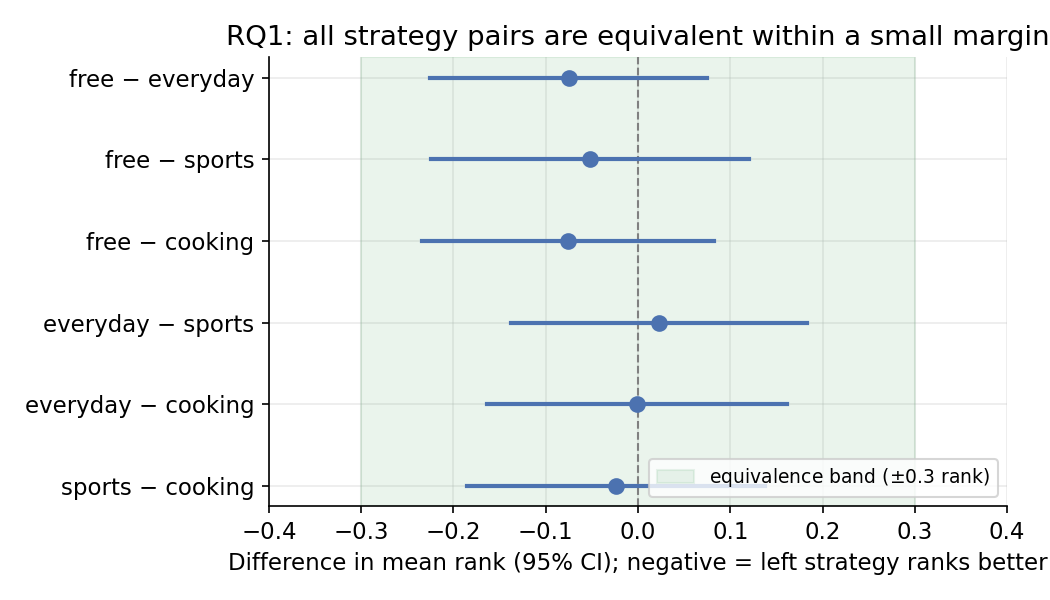
\includegraphics[width=0.78\linewidth]{rq1_equivalence.png}
\caption{RQ1: pairwise differences in mean rank between strategies (points) with 95\%
confidence intervals ($n = 64$ concepts). Every interval lies entirely within the
$\pm0.3$-rank equivalence band (shaded), so the strategies are statistically \emph{equivalent},
not merely non-significantly different.}
\label{fig:equiv}
\end{figure}

The secondary absolute-scoring channel agrees that there is no real effect, but it is
instructive about \emph{how} small models score. Ranked by mean \emph{overall usefulness} on
the 1--5 rubric, the order is likewise flat and not significant (\emph{everyday} 4.08,
\emph{free} 4.02, \emph{sports} 4.01, \emph{cooking} 3.96; Friedman $\chi^2 = 3.67$,
$p = 0.30$). The two channels do trend toward different orderings, though: ranking mildly
favours the concise ``free'' strategy while absolute scoring mildly favours the wordier
``everyday'' one. The reconciliation is a \emph{verbosity bias} in absolute scoring: analogy
length correlates positively with the absolute score (Spearman $0.15$, $p < 10^{-11}$), and
the ``free'' analogies are the shortest on average (63 words, versus 72--74 for the
constrained strategies), so brevity is rewarded head-to-head but penalised when scoring one
analogy in isolation. Comparative ranking is the more trustworthy channel precisely because
it is not fooled by length; either way, RQ1's answer is the same: \emph{no source-domain
constraint gives a reliable quality advantage over letting the model choose.}

By subject, no ordering is stable across both evaluation channels and both dataset sizes, with
the partial exception that the unconstrained strategy is consistently among the best for
Physics (rank 2.42). Subject ``winners'' otherwise shift between the two protocols and between
the 32- and 64-concept datasets (Table~\ref{tab:rq1}), which is exactly what one expects when
the underlying differences are noise. Generator identity mattered as little as strategy: the
three open generators produced analogies of similar judged quality, so the findings are not an
artefact of one model's style.

\begin{table}[t]
\centering
\caption{RQ1: mean rank of each generation strategy (1 = best of four), overall and by
subject, pooled over judges and generators. Lower is better; the best strategy in each row
is in \textbf{bold}.}
\label{tab:rq1}
\small
\begin{tabular}{lcccc}
\toprule
 & free & everyday & sports & cooking \\
\midrule
Overall      & \textbf{2.45} & 2.53 & 2.50 & 2.52 \\
Physics      & \textbf{2.42} & 2.43 & 2.47 & 2.67 \\
Chemistry    & \textbf{2.40} & 2.62 & 2.56 & 2.42 \\
Mathematics  & 2.50 & 2.51 & \textbf{2.43} & 2.56 \\
Biology      & 2.47 & 2.57 & 2.53 & \textbf{2.44} \\
\bottomrule
\end{tabular}
\end{table}

\begin{figure}[t]
\centering
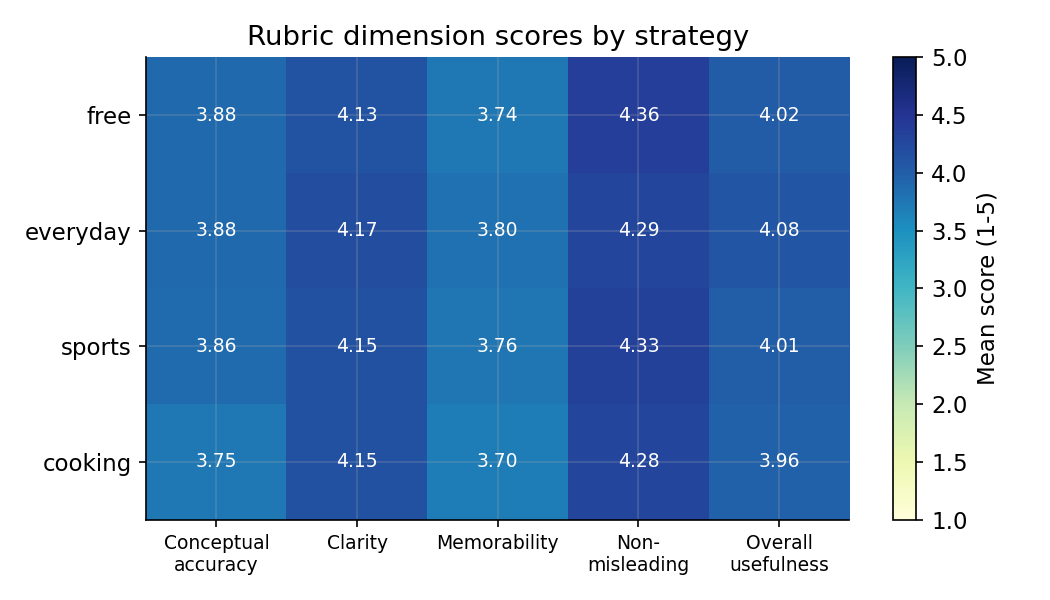
\includegraphics[width=0.82\linewidth]{rq1_dimension_heatmap.png}
\caption{Mean absolute rubric scores (1--5) by strategy and dimension, pooled over judges,
generators, and concepts. Scores cluster high (3.7--4.4) across every strategy and
dimension; this leniency, together with the length effect, makes absolute scoring an
unreliable discriminator of near-equal analogies.}
\label{fig:heatmap}
\end{figure}

\subsection{How well do the judges agree?}
\label{sec:results:agreement}
The two evaluation channels tell one consistent story about \emph{when} the panel is
reliable. Inter-judge agreement on the main comparison is very low (mean pairwise Spearman
correlation of 0.032 across judge-pairs and items for the rankings, and Krippendorff's
$\alpha$ between $-0.19$ and $0.12$ across the five rubric dimensions, 0.007 for overall
usefulness, for the absolute scores), even though the very same judges agreed almost
perfectly on the probe. The reconciliation is that agreement is bounded by the
true quality variance among the items being compared. The four strategies produce analogies
of similar quality, so there is little real signal for judges to agree on, whereas the
probe's planted-wrong analogies create a large signal every judge detects. Near-zero agreement among small automated judges
would be unremarkable on its own \citep{zheng2023judging}; the informative part is the contrast
with the same judges' unanimous agreement on the probe, which shows the low coefficient reflects
the items' narrow quality spread rather than broken judges. An agreement coefficient reported
without this context would be actively misleading, which is why we pair it with the probe. Practically, the panel should be used to \emph{screen out} bad analogies,
not to finely rank good ones.

\begin{figure}[t]
\centering
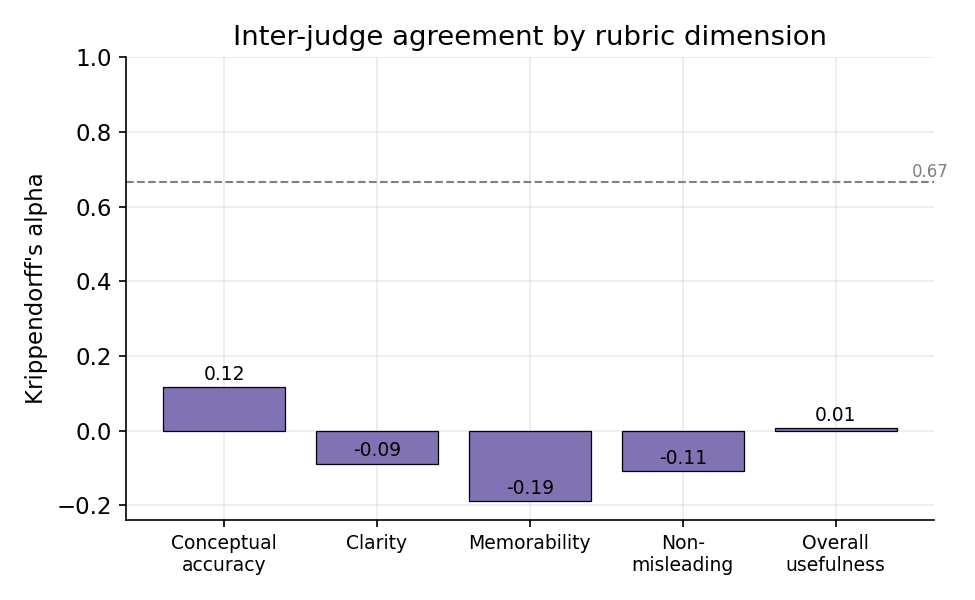
\includegraphics[width=0.72\linewidth]{rq1_interjudge_alpha.png}
\caption{Inter-judge agreement (Krippendorff's $\alpha$) on absolute rubric scores is near
zero or negative for every dimension, far below the 0.67 rule-of-thumb (dashed), even though
the same judges agree unanimously on the planted-quality probe. Agreement is bounded by the
true quality variance among the items compared.}
\label{fig:alpha}
\end{figure}

\subsection{What do the automated judges reward? (RQ2)}
\label{sec:results:rq2}
We read this predictor strictly as an audit of the judges: whatever predicts the judged score
is what the panel rewards, and, because the target is a judge score rather than a human rating,
a high $R^2$ diagnoses the evaluator rather than validating the analogies. An analogy's mean
judged usefulness turns out to be highly predictable from cheap surface features: a
random-forest regressor attains a five-fold cross-validated $R^2$ of 0.72 (mean absolute
error 0.13 on the 1--5 scale, $n = 1556$ analogies with judgements). \emph{What} it predicts
from is the revealing part. The dominant features are all measures of length and lexical
complexity (word count, proportion of long words, mean word length, readability, and words
per sentence), followed by grade level and subject, while the generation \emph{strategy}
contributes almost nothing (Figure~\ref{fig:rq2}). The automated quality score is therefore largely a function of how
long and lexically dense an analogy is, and of its subject, rather than of the pedagogical
strategy that produced it. This is the same verbosity bias that reconciles the two RQ1
channels (Section~\ref{sec:results:rq1}), now shown to be large enough to make quality
``predictable'' while being substantively about surface form. Verbosity and leniency biases in
automated judges are themselves well documented \citep{zheng2023judging}; the audit does not
rediscover them so much as show that, for the automated evaluation of instructional analogies,
they grow strong enough to dominate the quality signal, that they are worst in the small
models one can run locally, and (Section~\ref{sec:results:scale}) that they recede once the judge
is larger. The lesson is a caution, not a
capability: a predictor this accurate is tracking the judges' biases as much as the
analogies' merit, and any deployment that optimises analogies against such a score would be
optimising partly for length.

\begin{figure}[t]
\centering
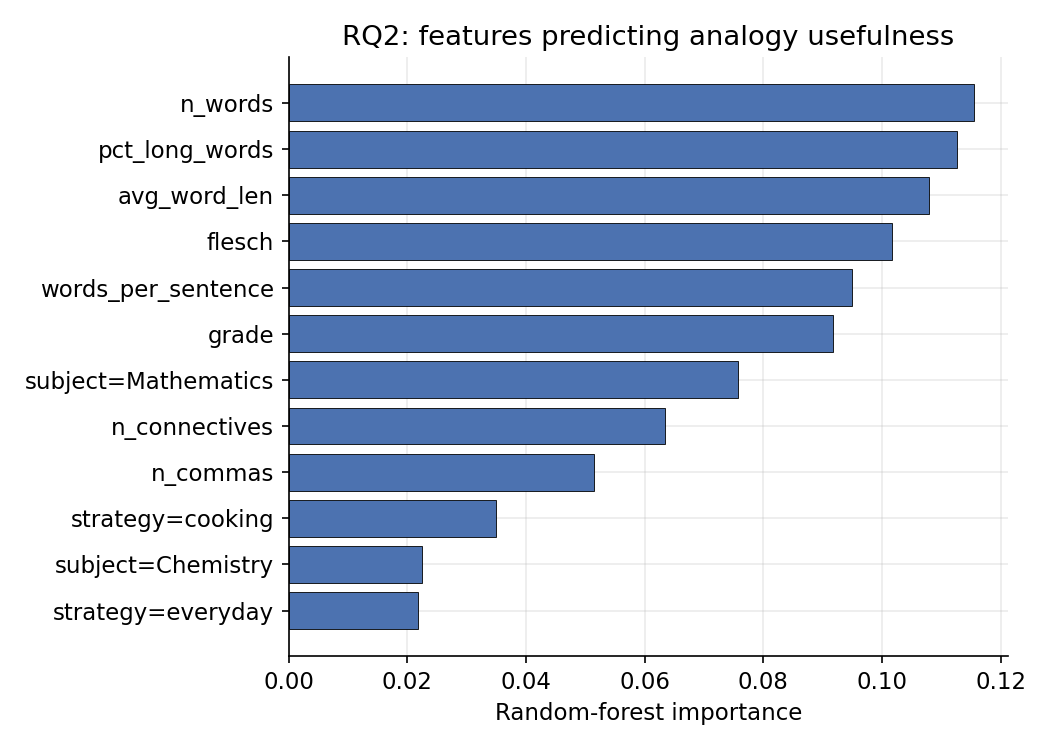
\includegraphics[width=0.82\linewidth]{rq2_feature_importance.png}
\caption{RQ2: random-forest feature importances for predicting an analogy's mean absolute
usefulness ($R^2 = 0.72$, five-fold CV). Surface length/complexity and subject dominate;
the generation strategy contributes little.}
\label{fig:rq2}
\end{figure}

\subsection{Do analogies help a student model? (RQ3)}
\label{sec:results:rq3}
It helps to be precise about what this test measures before reading anything into the numbers.
Holding the concept and its questions fixed, we ask whether prepending a teaching text changes a
model's objective multiple-choice accuracy. That is a test of whether the text carries
\emph{information the model can use to answer}, not a model of how a person learns; a claim about
human learning would need human learners, which is outside the scope of this fully automated study
(Section~\ref{sec:limitations}). Read in those narrower terms the measure still earns its place: if
an added analogy supplies no usable information beyond a plain explanation, that is at least a weak
mark against it, and it lines up with the quality findings above. The comprehension study first
establishes that the measure can detect a teaching effect at all, and then finds that analogies are
not where that effect comes from. Baseline accuracy
(question only, no teaching text) rises steeply with student capability (51.6\% for
Qwen2.5-0.5B, 63.3\% for Llama3.2-1B, and 92--94\% for the 2--3B models), so only the smaller
students have room to improve (Figure~\ref{fig:rq3}). Supplying the standard explanation
raises the weakest students sharply ($+15.6$ points for the 0.5B model and $+10.9$ for the 1B
model) while leaving the near-ceiling larger models essentially unchanged: a clean headroom
pattern that confirms the paradigm works. Adding an analogy \emph{on top of} that explanation,
however, produces no reliable improvement for any student. The analogy-minus-standard gain is
$+1.8$, $-0.4$, $+1.6$, and $-0.4$ points across the four models from weakest to
strongest, all within noise, and no prompting strategy stands out within the analogy
conditions. The comprehension benefit our method can detect therefore comes from the
explanation, not from the analogy layered on top of it. This dovetails with RQ1 (the
analogies are not strongly differentiated in quality) and with the human-subjects finding that
LLM analogies help learners chiefly after a teacher curates them \citep{shao2025unlocking}: raw,
automatically generated analogies do not, on their own, move a proxy learner's comprehension
beyond a plain explanation.

\begin{figure}[t]
\centering
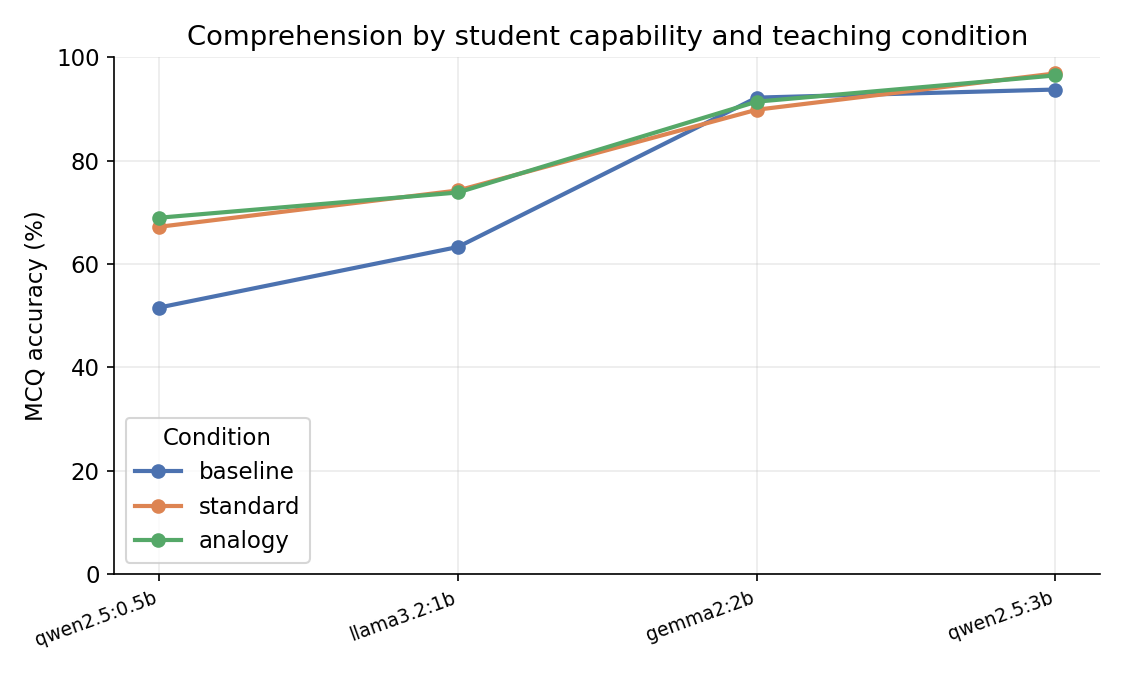
\includegraphics[width=0.85\linewidth]{rq3_capability_gradient.png}
\caption{RQ3: multiple-choice accuracy by student model (increasing capability, left to right)
and teaching condition. A standard explanation (orange) lifts the weak students well above
baseline (blue), but adding an analogy (green) tracks the explanation almost exactly at every
capability level, and all conditions converge at the ceiling for the 2--3B students.}
\label{fig:rq3}
\end{figure}

\subsection{Does it replicate in Hindi? (RQ4)}
\label{sec:results:rq4}
Repeating the pipeline in Hindi separates a \emph{finding} that seems to carry across languages
from \emph{tooling} that plainly does not. The substantive result is at least consistent across
languages: over the 20 paired concepts the four strategies are again statistically
indistinguishable (Friedman $\chi^2 = 1.95$, $p = 0.58$). We read this as suggestive rather than a
firm replication, and the rest of the section is why: the Hindi panel parses and discriminates so
poorly that a small strategy effect, had one been present, could easily have been lost in the noise
rather than truly absent. The result we can state without reservation is the negative one about the
tooling, which degrades sharply (Table~\ref{tab:hindi}). First, the panel's output
stops being well-formed: only 55\% of Hindi ranking prompts and 35\% of Hindi rubric-scoring prompts
return parseable output, against 94\% and 97\% in English, because the small models frequently lapse
into commentary, mix scripts, or abandon the requested format in Hindi. Second, and more seriously,
the judges largely lose the ability to tell good analogies from bad: on the Hindi validation probe
the planted-wrong analogy is ranked below the correct one only 58\% of the time, barely above the
50\% chance level, versus 100\% in English, and the clean good $<$ decent $<$ vague $<$ wrong
ordering collapses. Inter-judge agreement is no better than in English (Spearman $-0.18$), and the
verbosity bias does not clearly reappear, though that last comparison rests on the thin 35\% of
Hindi scores that parsed at all.

The reading is cautionary and, we think, useful. At this model scale the automated screening
protocol is largely an \emph{English} capability: the claim it establishes for English, that
source-domain constraints do not help, appears to hold in Hindi too, though with the caveat just
noted that a panel this degraded could as easily be masking a small effect, and in any case the
panel that establishes it can no longer be trusted to screen Hindi analogies. Deploying such a pipeline for Hindi, and by extension
for other mid- and low-resource languages, would need either stronger multilingual models or a human
in the loop. Reporting this breakdown honestly is more useful to a practitioner than a figure showing
that the protocol nominally ``ran'' in Hindi.

\begin{table}[t]
\centering
\caption{Cross-lingual comparison (RQ4). The no-strategy-effect finding appears to hold in Hindi,
but the automated evaluation degrades sharply: output stops parsing and the judges stop
discriminating quality, so the apparent replication is read cautiously. Hindi covers a paired
20-concept subset.}
\label{tab:hindi}
\small
\begin{tabular}{lcc}
\toprule
 & English & Hindi \\
\midrule
Ranking output parseable               & 94\% & 55\% \\
Rubric output parseable                & 97\% & 35\% \\
Strategy effect (Friedman $p$)         & 0.72 & 0.58 \\
Probe: wrong ranked below good         & 100\% & 58\% \\
Inter-judge agreement (Spearman)       & 0.03 & $-0.18$ \\
Length--score correlation (verbosity)  & $+0.15$ & $-0.09$ \\
\bottomrule
\end{tabular}
\end{table}

\subsection{Does it hold with a larger judge?}
\label{sec:results:scale}
Because every panel model is small (0.5--3.8B parameters), we re-ran the full evaluation with a
larger judge, qwen2.5-7B (roughly twice the panel's size), over all 64 concepts (192 rankings,
768 absolute scores) and the probe. Two findings replicate and two are \emph{sharpened}, and the
sharpening runs in the direction of the small panel being the limitation rather than the result.
Replicating: the larger judge screens the planted-wrong probe analogies perfectly (100\%) and
produces cleaner output (100\% parse, versus the panel's 97\%). Sharpened: first, the verbosity
bias essentially \emph{vanishes} (the length--score correlation falls from $+0.15$ to $-0.02$),
and with it the disagreement between the two evaluation channels; the 7B judge rates the concise
``free'' strategy highest in both ranking and absolute scoring, so the channel divergence we saw
with small judges was itself a symptom of their length bias. Second, and more consequentially, the
larger judge \emph{resolves} a modest strategy ordering the small panel could not: it ranks free
best and cooking worst, and a Friedman test is now significant ($\chi^2 = 22.3$, $p = 0.0001$,
$n = 64$). The direction matches the small panel's non-significant trend (free best in the
ranking channel), so the reading is not that source domain suddenly matters, but that a cleaner
judge detects a small real advantage for unconstrained generation that a lenient small panel
washes out into apparent equivalence. Frontier-scale judges remain untested (we use no paid API),
but the trajectory is consistent: better judges screen as well, shed the verbosity bias, and
mildly favour letting the model choose its own analogy, exactly the practical guidance of
Section~\ref{sec:results:rq1} (Table~\ref{tab:scale}). The picture is symmetric on the
generation side: when the larger 7B model instead \emph{writes} the analogies, the small panel
still finds no strategy effect among them (Friedman $p = 0.40$, free best), and the same length
pattern holds (free is the most concise, at 52 words). So neither the no-effect finding nor the
length confound is an artefact of using small \emph{generators} either.

\begin{table}[t]
\centering
\caption{The findings under a larger judge: the small panel (0.5--3.8B) versus a single 7B judge over
the full 64 concepts. The larger judge screens as well, but it sheds the small-model verbosity
bias, agrees across its two channels, and resolves a strategy effect the panel cannot.}
\label{tab:scale}
\small
\begin{tabular}{lcc}
\toprule
 & Small panel & 7B judge \\
\midrule
Probe: wrong analogy caught       & 100\% & 100\% \\
Output parseable                  & 97\%  & 100\% \\
Strategy effect (Friedman $p$)    & 0.72  & $<0.001$ \\
Verbosity (length--score $r$)     & $+0.15$ & $-0.02$ \\
Best strategy (ranking / absolute)& free / everyday & free / free \\
\bottomrule
\end{tabular}
\end{table}

\section{Discussion}
\label{sec:discussion}

\paragraph{Prompting: let the model choose the domain.}
The clearest practical message from RQ1 is a negative one, and negative results are useful
here precisely because the intuition they overturn is so common. Constraining the analogy's
source domain does \emph{not} reliably produce better analogies than simply asking for the
best analogy the model can think of. The evidence for ``no reliable effect'' is unusually
direct: neither evaluation protocol finds a significant strategy effect (Friedman $p = 0.72$
for ranking and $p = 0.30$ for absolute scoring, at $n = 64$ concepts), and the mild orderings
they do produce point in opposite directions (comparative ranking favours the concise
unconstrained ``free'' strategy, absolute rubric scoring the wordier ``everyday'' one), a
divergence we trace to a verbosity bias in the small judges rather than to any genuine
quality gap (Sections~\ref{sec:results:rq1} and~\ref{sec:results:rq2}). Under the small panel
the four strategies are statistically equivalent within a small margin. A larger, cleaner judge
(Section~\ref{sec:results:scale}) refines rather than overturns this: it sheds the length bias,
its two channels agree, and it resolves a modest but significant advantage for the unconstrained
strategy. Both readings point the same way: what survives is that
leaving the domain unconstrained is at least as good as any constraint, and by the better judge
mildly the best, while producing shorter analogies, so the practical guidance is to let a capable model pick the source domain
by default and to reach for a specific domain only where the subject makes a mapping obviously
natural (as for Physics, the one subject in which ``free'' wins under both protocols). This
fits the structure-mapping view that what matters is whether the base's relational structure
maps onto the target, not which corner of everyday life it is drawn from
\citep{gentner1983structure}.

\paragraph{Automated evaluation screens well but ranks poorly.}
The single most important methodological finding is the gap between two things people
routinely conflate when they report ``LLM-judge agreement.'' On our validation probe,
where one analogy in each set is deliberately wrong, every judge places the wrong analogy
below the correct one essentially always, and the panel's tier ordering is exactly right.
On the main comparison, where four reasonable strategies produce analogies of genuinely
similar quality, inter-judge agreement collapses toward zero. Both facts are true of the
same judges at the same time; the difference is entirely in how much real quality variance
there is to detect. The lesson is that a panel of small models is trustworthy as a
\emph{screen}, for catching analogies that are actually wrong or misleading, but should
not be over-interpreted as a fine-grained ranker of near-equal candidates, and that a bare
agreement coefficient is meaningless without stating the quality spread of the items it was
computed over. This is why we report the probe alongside the agreement statistics rather
than either one alone.

\paragraph{Comprehension gains live where the learner has headroom.}
Tying quality to a behavioural outcome exposes a third pattern: whether added explanation
or analogy helps at all depends on the ``student.'' A capable model already answers our
conceptual questions correctly without any teaching text and therefore cannot show a gain,
whereas smaller models have the headroom for teaching material to matter
(Section~\ref{sec:results:rq3}). In our data the standard explanation raised the weakest
model's accuracy by roughly sixteen points while leaving the ceilinged models flat, yet adding
an analogy on top of the explanation produced no reliable gain for any model, so even the
comprehension effect we \emph{can} detect is attributable to the explanation rather than to
the analogy. The methodological implication generalises beyond our setting: using
an over-competent model as a proxy learner will systematically \emph{understate} the value
of any instructional intervention, and studies that use LLMs as stand-in students should
report the proxy's baseline competence for exactly this reason.

\paragraph{A reusable, honest protocol.}
Taken together, the pieces form a template that others can run on commodity hardware: fix
the concept content, vary only the generation prompt, rank rather than absolutely score,
shuffle to defeat position bias, exclude self-judgements, and, above all, validate the
judges against planted known-quality items before trusting any number they produce. None of
these steps requires a paid API or a human rater, which makes the protocol cheap enough to
use as a first-pass filter in an actual content pipeline, with humans reserved for the
close calls the automated panel cannot resolve.

\paragraph{Implications for educational practice and technology.} For the different stakeholders in
education, the results translate into concrete guidance. For a \emph{teacher} or content author the
message is permissive: a capable model's own choice of analogy domain is, on average, as good as a
hand-specified one, so effort is better spent curating and checking a few candidates than engineering
elaborate ``use a sports analogy'' prompts. For an \emph{educational-technology team} building an
analogy feature, a panel of small open models is a usable and essentially free quality \emph{gate}: it
reliably filters out wrong and misleading analogies before they reach a learner, and its cost profile
(no paid API, one commodity GPU) makes it deployable at scale, provided it is treated as a screen and
validated against known-quality anchors rather than trusted as a fine-grained ranker. For an
\emph{institution or regulator} vetting automatically generated material, the study offers both a
reusable rubric and a candid map of where automated evaluation is trustworthy (catching clear errors)
and where it is not (splitting hairs among already-good analogies, or working outside English). And
for \emph{learners in mid-resource languages}, the Hindi result is a caution: the same automated
safeguards that protect English content do not yet transfer, so human oversight remains essential
wherever the tooling is weakest.

\section{Limitations and threats to validity}
\label{sec:limitations}
Several limitations bound our claims, and we state them plainly because the paper's value depends on
being honest about what automated evaluation can and cannot do. Each is numbered so that
Section~\ref{sec:future} can pair it, one to one, with a corresponding avenue of future research.

\emph{L1. Proxies for people.} The judges and the ``students'' are language models standing in for
human teachers and learners, and this is the paper's central scope limitation: absent human ratings,
our quality and comprehension numbers are automated proxy measurements. Two of the four measurements
are, deliberately, \emph{not} one model judging another. The judge-validation probe scores each panel
against planted analogies of \emph{known}, author-fixed quality (including analogies that are
objectively wrong), so it measures discrimination against ground truth; and the comprehension study
(RQ3) scores multiple-choice answers objectively against fixed keys. The learner is still a model,
however, so RQ3 is best read as measuring whether a teaching text carries information a model can
\emph{use}, and it bears on human learning only indirectly. These objective anchors let us state the
paper's firmest claims without resting them on one model rating another; the remaining subjective
judgements (the rubric panel) are reported throughout with their agreement caveats.

\emph{L2. Small-model judging.} Our judges are 2--3.8B-parameter models chosen to run on a 4\,GB GPU.
They are lenient, they disagree on near-equal items, and, before we shuffled labels and switched to
ranking, some defaulted to presentation order rather than reading the analogies. We mitigate these
behaviours and validate against a probe, and our larger-judge check (Section~\ref{sec:results:scale})
bears this out in part: at 7B the screening and no-effect findings replicate and the verbosity bias
weakens. Frontier-scale judges remain untested, so some quantitative details (the exact agreement
levels and the size of the verbosity bias) may be specific to this model scale.

\emph{L3. Scope of the dataset.} We study 64 concepts across four subjects at grades 8--12, with a
16-concept multiple-choice subset. This is enough to detect subject-level patterns but is far from
full curriculum coverage, and the concepts, explanations, and questions were authored by a single
researcher, which may embed idiosyncratic choices. The parts that serve as \emph{ground truth},
however, are objective: the multiple-choice keys are verifiable curriculum facts and the probe's
planted-wrong analogies contain clear, checkable errors.

\emph{L4. Cross-lingual scope.} The Hindi replication covers a single language, 20 concepts, and a
code-mixed register, and the low Hindi parse rates mean that some Hindi metrics (notably the
absolute-scoring comparisons, computed on the 35\% of outputs that parsed) rest on limited data. It
establishes that the automated protocol degrades sharply outside English, but not precisely how it
would behave for other languages or scripts, and the apparent replication of the no-effect finding in
Hindi is therefore best read as exploratory.

\emph{L5. Generator/judge overlap and self-preference.} Three of the four panel models also serve as
generators. We exclude every model from judging its own analogies, which removes direct
self-preference, but shared training lineages could still induce subtler family-level preferences that
our design does not fully rule out.

\emph{L6. Rubric validation.} SAQR is grounded in the learning-sciences literature and is
behaviourally validated only indirectly (through the discrimination probe and the comprehension
study). A formal validation against expert human ratings, and a test of its dimensions' independence,
are not attempted here.

\section{Avenues of Future Research}
\label{sec:future}
We map each limitation above to a concrete next step, one to one, so that the research agenda follows
directly from the boundaries of the present study.

\emph{FR1 (addresses L1).} Conduct a human validation study: have expert teachers rate a sample of the
generated analogies and have students take the comprehension test, then calibrate the automated proxy
measurements against those human judgements. This is the single most important step for turning the
protocol's proxy screen into evidence about human learning, and for an educational-technology team it
is the study that would justify placing automated screening in front of real learners.

\emph{FR2 (addresses L2).} Repeat the protocol with progressively larger and frontier judges to
establish how inter-judge agreement, discrimination, and the verbosity bias scale with judge size, and
so to locate the reliability ceiling. For a product team this quantifies the cost-reliability
trade-off between a free small-model screen and a paid larger judge.

\emph{FR3 (addresses L3).} Expand to full-curriculum coverage authored by multiple subject-matter
experts, enabling per-topic and cross-author analyses and reducing single-author idiosyncrasy. This is
what a curriculum body or textbook publisher would need before treating the protocol as a system-wide
quality gate.

\emph{FR4 (addresses L4).} Extend the cross-lingual study to more languages and scripts, with improved
parsers or lightly instruction-tuned judges to raise parse rates, and map precisely where the protocol
holds and where it fails. This directly targets the equity gap the Hindi arm surfaced.

\emph{FR5 (addresses L5).} Use judge models drawn from disjoint training lineages, or held-out judges
that never serve as generators, to rule out family-level preferences and further harden the panel
against self-preference.

\emph{FR6 (addresses L6).} Formally validate SAQR against expert human ratings and test the
statistical independence of its five dimensions, yielding a rubric that other researchers and edtech
teams can adopt with calibrated confidence.

\section{Conclusion}
\label{sec:conclusion}
We set out to answer two coupled questions about instructional analogies in the age of
language models: how to prompt for good ones, and how to judge them at scale, using only a
protocol cheap and reproducible enough to run on a single consumer GPU with no paid API and
no human annotation. The prompting answer is deflationary but useful: constraining
the analogy's source domain does not reliably beat letting a capable model choose for
itself, and domain constraints help only where the subject makes a particular mapping
natural. The evaluation answer is more consequential. A panel of small open models is a
valid \emph{screen}: it detects wrong and misleading analogies almost perfectly, as our
planted-quality probe shows, but it is not a reliable fine-grained ranker of analogies that
are already good, and its inter-judge agreement is meaningful only when read against the
quality spread of the items being compared. Coupled with the finding that an over-competent
model masks comprehension gains that only appear once the learner has headroom, the overall
message is that automated evaluation of instructional content is genuinely usable, but only
when it is validated against known-quality anchors and its limits are stated rather than
hidden. Scaling the judge is the clearest lever for reliability: our larger-model check sheds
the small models' verbosity bias and resolves quality differences the small panel cannot. A
Hindi replication draws that boundary sharply: the no-effect finding holds across
languages, but the automated panel that establishes it parses and discriminates reliably only
in English at this model scale, so the protocol is, for now, an English-first tool. We release
the concept dataset, the SAQR rubric, all prompts, code, and raw model
outputs so that the protocol, and its honest accounting of what it can and cannot
measure, can be reused and stress-tested.

\bibliographystyle{plainnat}
\bibliography{refs}

\appendix
\section*{Supplementary material}
\addcontentsline{toc}{section}{Supplementary material}
\noindent The following appendices (the full SAQR rubric, the concept dataset, the prompt templates,
and worked example analogies and judgments) are provided as supplementary material. They document and
support the study but are not essential to the main argument, and can be moved to an online supplement
in line with the target journal's policy.

\section{The SAQR rubric in full}\label{app:rubric}
Each dimension is scored from 1 to 5 (1 = absent/poor, 2 = weak, 3 = adequate, 4 = good, 5 = excellent). Use the full range; reserve 5 for genuinely excellent cases and give low scores where the analogy is weak.

\paragraph{Conceptual accuracy (\texttt{conceptual\_accuracy}).} Does the analogy map correctly onto the target concept, so that the important relationships in the concept correspond to matching relationships in the analogy?
\emph{1:} The analogy is wrong or maps to the wrong idea; following it would teach an incorrect concept. \quad \emph{3:} The analogy captures the main relationship correctly, with minor gaps. \quad \emph{5:} The analogy maps the key relationships of the concept faithfully and precisely.

\paragraph{Clarity (\texttt{clarity}).} Would a school student find the analogy easy to follow, and does it actually make the concept easier to grasp than the bare explanation?
\emph{1:} Confusing or harder to follow than the concept itself. \quad \emph{3:} Clear and does help understanding. \quad \emph{5:} Immediately clear and noticeably illuminates the concept.

\paragraph{Memorability (\texttt{memorability}).} Is the analogy vivid, concrete, and relatable enough that a student is likely to remember it and, through it, the concept?
\emph{1:} Bland or abstract; nothing to hold onto. \quad \emph{3:} Concrete and reasonably sticky. \quad \emph{5:} Vivid, concrete, and highly memorable.

\paragraph{Absence of misleading simplification (\texttt{non\_misleading}).} Does the analogy avoid introducing misconceptions? A good analogy either does not break down in a harmful way, or its limits are not likely to mislead a student.
\emph{1:} Introduces a clear misconception a student would plausibly carry away. \quad \emph{3:} Mostly safe; minor over-simplification unlikely to mislead. \quad \emph{5:} No misleading simplification; the analogy breaks down only in ways a student would not over-extend.

\paragraph{Overall usefulness (\texttt{overall\_usefulness}).} All things considered, how useful is this analogy for teaching this concept to a school student?
\emph{1:} Not useful; better to omit it. \quad \emph{3:} Useful; a fair teacher would include it. \quad \emph{5:} Highly useful; a strong teaching aid.

\section{Concept dataset}\label{app:concepts}
The 32 concepts, balanced across four subjects and grades 8--12. Concepts marked $\star$ carry the four-option multiple-choice items used in the comprehension study.
\begin{center}\small
\begin{tabular}{llcl}
\toprule
ID & Subject & Grade & Concept \\ \midrule
bio\_osmosis & Biology & 9 & Osmosis across a semipermeable membrane $\star$ \\
bio\_enzyme & Biology & 10 & Enzymes as biological catalysts $\star$ \\
bio\_photosynthesis & Biology & 10 & Photosynthesis  \\
bio\_homeostasis & Biology & 11 & Homeostasis and negative feedback $\star$ \\
bio\_mitosis & Biology & 11 & Mitosis (cell division)  \\
bio\_neuron & Biology & 11 & Nerve impulse and the action potential  \\
bio\_dna\_replication & Biology & 12 & DNA replication  \\
bio\_natural\_selection & Biology & 12 & Natural selection $\star$ \\
che\_mole & Chemistry & 9 & The mole as a counting unit $\star$ \\
che\_covalent\_bond & Chemistry & 10 & Covalent bonding  \\
che\_exothermic & Chemistry & 10 & Exothermic and endothermic reactions  \\
che\_ph & Chemistry & 10 & The pH scale for acids and bases $\star$ \\
che\_catalyst & Chemistry & 11 & Catalysts and activation energy $\star$ \\
che\_equilibrium & Chemistry & 11 & Dynamic chemical equilibrium $\star$ \\
che\_ideal\_gas & Chemistry & 11 & The ideal gas law  \\
che\_redox & Chemistry & 11 & Oxidation and reduction (redox)  \\
mat\_slope & Mathematics & 9 & Slope of a straight line $\star$ \\
mat\_probability & Mathematics & 10 & Basic probability of independent events $\star$ \\
mat\_derivative & Mathematics & 11 & The derivative as an instantaneous rate of change $\star$ \\
mat\_function & Mathematics & 11 & Functions, domain and range  \\
mat\_logarithm & Mathematics & 11 & Logarithms  \\
mat\_vectors & Mathematics & 11 & Vectors as magnitude and direction  \\
mat\_integral & Mathematics & 12 & The definite integral as accumulated area $\star$ \\
mat\_matrix & Mathematics & 12 & Matrices and matrix multiplication  \\
phy\_pressure & Physics & 8 & Pressure as force per unit area  \\
phy\_newton3 & Physics & 9 & Newton's third law of motion $\star$ \\
phy\_ohm & Physics & 10 & Ohm's law and electrical resistance $\star$ \\
phy\_refraction & Physics & 10 & Refraction of light  \\
phy\_gravitation & Physics & 11 & Newton's law of universal gravitation  \\
phy\_momentum & Physics & 11 & Momentum and its conservation  \\
phy\_resonance & Physics & 11 & Resonance in oscillating systems $\star$ \\
phy\_induction & Physics & 12 & Electromagnetic induction (Faraday's law) $\star$ \\
\bottomrule
\end{tabular}
\end{center}
\section{Prompts}\label{app:prompts}
\paragraph{Analogy generation (system).} \small\ttfamily You are an expert STEM teacher. You explain a concept with ONE vivid analogy that a school student (Class 8 to 12) can understand. The analogy must be scientifically faithful: the important relationships in the concept must correspond to matching relationships in the analogy. Do not teach a misconception for the sake of simplicity.\normalfont\normalsize
\paragraph{Generation strategy instructions.}\begin{itemize}\setlength\itemsep{0pt}
\item \textbf{free}: Use the single best analogy you can think of, from any source domain.
\item \textbf{everyday}: Use an analogy drawn from ordinary everyday life (the home, daily routines, common objects).
\item \textbf{sports}: Use an analogy drawn from sports, games, or physical play.
\item \textbf{cooking}: Use an analogy drawn from cooking, baking, or the kitchen.
\end{itemize}
\paragraph{Comparative ranking (system).} \small\ttfamily You are an experienced STEM teacher comparing teaching analogies. You will see several analogies for the SAME concept, each labelled with a letter. Rank them from best to worst as teaching aids for a school student (Class 8 to 12), judging conceptual accuracy, clarity, and whether they mislead. Output ONLY lines of the form 'LETTER: rank', one per analogy, where 1 is best. Use each rank exactly once. No commentary.\normalfont\normalsize
\paragraph{Absolute rubric scoring (system).} \small\ttfamily You are an experienced STEM teacher evaluating a teaching analogy on a fixed rubric. Score each dimension from 1 to 5 as a whole number, using the full range: 1 is poor, 3 is adequate, 5 is excellent. Do not give every dimension the same high score; discriminate. Output ONLY lines of the form 'dimension\_key: score', one per dimension, no commentary.\normalfont\normalsize


\section{Example analogies and judgments}
\label{app:examples}

\paragraph{Judge validation (a probe item).} For the Ohm's-law probe, the panel's mean ranks
(1 = best of four) were \emph{good} 1.33, \emph{decent} 2.00, and the \emph{vague} and
\emph{wrong} analogies tied at 3.33; every judge placed the wrong analogy below the correct
one. (Aggregated over all five probe concepts the ordering is strict: 1.79 / 1.95 / 2.63 /
3.63.) The four planted analogies were:
\begin{description}[leftmargin=0pt,itemsep=1pt]
  \item[\textnormal{\emph{good} (1.33):}] ``Voltage is like the water pressure in a pipe,
    current is the rate at which water flows, and resistance is how narrow the pipe is: for a
    fixed pressure, a narrower pipe lets less water flow, so the current is smaller.''
  \item[\textnormal{\emph{decent} (2.00):}] ``A circuit is like people walking down a
    corridor. Voltage is how hard they are pushed from behind and resistance is how narrow the
    corridor is.''
  \item[\textnormal{\emph{vague} (3.33):}] ``Electricity is a bit like a river: it just flows
    along from one place to another.''
  \item[\textnormal{\emph{wrong} (3.33):}] ``Resistance is like adding an extra battery to the
    circuit. The more resistance you add, the harder it pushes the charges, so a higher
    resistance always makes a larger current flow.'' (This inverts Ohm's law.)
\end{description}

\paragraph{Generated analogies and the two channels.} For the same concept, the analogies
Qwen2.5-3B generated show the absolute-versus-ranking disagreement in miniature. The concise
\emph{free} analogy, ``Resistance is like a dam in a river system; more resistance means
water (current) slows down and flows less even if pressure (voltage) remains constant'', drew
the \emph{highest} absolute usefulness (4.67/5) yet a worst-tied mean rank (2.67), whereas the
wordier \emph{everyday} ``traffic jam'' analogy scored lower in isolation (4.33) but ranked
best (2.33). Brevity is rewarded head-to-head and penalised when scoring one analogy at a
time: the verbosity bias of Section~\ref{sec:results:rq2} in a single example.

\end{document}
